
\documentclass[sigconf,authordraft, nonacm=true]{acmart}

%%
%% \BibTeX command to typeset BibTeX logo in the docs
\AtBeginDocument{%
  \providecommand\BibTeX{{%
    \normalfont B\kern-0.5em{\scshape i\kern-0.25em b}\kern-0.8em\TeX}}}

\begin{document}

%%
%% The "title" command has an optional parameter,
%% allowing the author to define a "short title" to be used in page headers.
\title{Deep reinforcement learning based multi-agent pathway finding}

\author{Luo Zhiyao}
\author{under the supervision of Prof. Guillaume Adrein Sartoretti}
\email{A0209423L}
\email{e0452733@u.nus.edu}

\affiliation{%
  \institution{Multi-Agent Robotic Motion Laboratory}
  \city{National University of Singapore}
  \postcode{Singapore 119077}
}

%%
%% The abstract is a short summary of the work to be presented in the
%% article.
\begin{abstract}
  Multi-agent pathway finding (MAPF) is a significant topic of many large-scale robotic applications from logistic distribution system to Simultaneous localization and mapping. Guillaume Sartorretti et ai proposed PRIMAL framework. It casts MAPF into reinforcement learning framework where agents are expected to learn full-decentralized policies under the demonstration of expert system. This paper extends the previous work on PRIMAL to 3D search space and discusses the communication mechanism between agents. We present results on randomized worlds with same settings on original PRIMAL, and compare success rate against original PRIMAL. By careful reward shaping and gradient clipping, introducing communication into PRIMAL make imitation loss convergence steadily to a relatively low value and effectively improve the effort of expert demonstration, which lead to more optimal pathway planning than original PRIMAL. 
\end{abstract}


%%
%% Keywords. The author(s) should pick words that accurately describe
%% the work being presented. Separate the keywords with commas.
\keywords{datasets, neural networks, gaze detection, text tagging}

\maketitle

\section{Introduction}


\section{Prior Work}
\subsection{Multi-agent path finding}
Multi-agent path finding (MAPF) is a classical problem in planning and has been studied extensively (Ma et al. 2017a; Felner et al. 2017). Given a set of agents, MAPF consists in finding, for each agent, a path from its start location to its goal while avoiding collisions between agents. Collisions occur when two agents simultaneously occupy the same location or simultaneously cross the same edge in opposite directions. This problem has applications in contexts as diverse as warehouse logistics (Wurman, D’Andrea, and Mountz 2008), video games (Silver 2005), and even search and rescue (Kitano et al. 1999). 

\subsection{decoupled, centralized and dynamic decoupled system}


\subsection{Pathfinding via Reinforcement and Imitation Multi-agent Learning(PRIMAL)}

{\itshape template style}



\subsection{M$^*$}


{\bfseries Your document will be returned to you for revision if
  modifications are discovered.}

\section{Assumptions}
\subsection{Search Space}
In this paper, MAPF problem is discussed in discrete space (2D or 3D), where the environment can be represented by a grid world. an Agent, an obstacle block and a goal point occupy respectively a unit grid (1 by 1 in 2D space, 1 by 1 by 1 in 3D space) in the environment. An example of discrete MAPF environment is shown in fig.  
\\We assume that agents can move in the 4-connected region. In 2D space, considering an agent located at position (x${_0}$, y${_0}$), it has maximum 4 valid actions (up, down, left, fight), which would result in the state transition to (x${_0}$, y${_0}$+1), (x${_0}$, y${_0}$-1), (x${_0}$-1, y${_0}$), (x${_0}$+1, y${_0}$) correspondingly. Whilst in 3D space, an agent has maximum 6 valid actions along both positive and negative directions of axis x, y and z, which will respectively transit the original state (x${_0}$, y${_0}$, z${_0}$) to (x${_0}$+1, y${_0}$, z${_0}$), (x${_0}$-1, y${_0}$, z${_0}$), (x${_0}$, y${_0}$,+1 z${_0}$), (x${_0}$, y${_0}$-1, z${_0}$), (x${_0}$, y${_0}$, z${_0}$+1) and  (x${_0}$, y${_0}$, z${_0}$-1). We also assume that all the agents move at the same speed, i.e. 1 unit cell per time step.  

\subsection{Collision}  
Collisions between agents occur when two agents simultaneously occupy the same location or simultaneously cross the same edge in opposite directions. It is also possible that agents collide with obstacles, or hit the boundary of environment. When the collision occurs in the above-mentioned conditions, the colliding agents will be forced to remain its state unchanged instead of taking its action in the next step. The action which will result in any collision next step is denoted as an invalid action. Fig demonstrates two particular cases that agents are allowed or prevented to perform their actions.

\subsection{MAPF environment realization in Python}
Since the MAPF environment we define is discrete, we can represent the entire state space as a double-layer matrix, which will be further discussed in section.  The environment is centralized, with a set of functions responsible for the interactions with agents. Environment is initialized with a world map that contains all the state information of agents, obstacles and goals. At the start of a time step, environment assigns observation arrays to all the agents according to the current states of the agents. Then agents make their decisions to determine where they would go at the next time step based on the observation received from the environment. The actions that agents make will correspondingly be sent to verify validation by the environment. The environment will automatically replace any invalid actions that agents may decide to take with standing still, and corresponding penalty on agents’ rewards will be dealt. After proceeding all the actions of the agents, environment finally allows agents to transit to the next state. The pseudo code of centralized environment is shown in fig.

\section{3D representation of PRIMAL}

In this section, we present how the MAPF problem is fit into the reinforcement learning framework in 3D space. We will demonstrate the observation and action space of each agent, the reward structure and the neural network that represents the policy to be learned comparing with 2D PRIMAL.

\subsection{Observation space}
The first layer is called state map, where agents are denoted by its agent ID, obstacles are denoted by -1, free space denoted by 0, and the second layer is the goals map, where goals are denoted by the agent ID it belongs to.
Considering a partially-observable discrete grid world where agents can only observe the state of the world in a limited field of view centered around themselves (11 by 11 by 11 field of view in practice), the observation of each agent consists of 4 layers of sub-observation respectively containing obstacle position, neighbor agents’ positions, neighbors’ goals and agent’s goal to simplify the learning task. All the four sub-observations are binary. When agents are close to the edges of the world, obstacles are added at all positions outside the world’s boundaries.
\\We believe that partial observation is critical to PRIMAL especially in 3D case. Since the dimension of observation expands from 3 to 4 (4*11*11 to 4*11*11*11) while obstacle density remains unchanged, the observation information would become highly sparse. To decrease the input dimension and reduce the possibility of divergence, setting observation size equal to 11*11*11 is effective experimentally.
Besides, agent needs to have access to information about its goal, which is often outside of its field of view in partial-observation case. We provide each agent both a unit vector pointing towards its goal and Euclidean distance to tis goal at all times. 

\subsection{Action space}
Agents take discrete actions the grid world: moving one cell in one of the six cardinal directions in 3D space (forward, back, up down, left right) or staying still. During training, actions are sampled only from valid actions and an additional loss functions aids in learning this information. In other words, all the invalid actions will be filtered by the environment. This will experimentally enable more stable training, compared to giving punishment for selecting invalid moves. 
\\If an agent selects an invalid move during testing, it instead says still for that timestep, and corresponding penalty will be dealt. In practice, agents very rarely select invalid moves once fully trained, showing that they effectively learn the set of valid actions in each state.
\\Additionally, to combat convergence to oscillating policies, agents are prevented during training from returning to the location they occupied at the last time step but agents can still stay still during multiple successive time steps, which is to guarantee agents a way to turn back if it is a must. This is necessary to encourage exploration and learn effective policies even during M${_*}$ imitation learning process.

\subsection{Reward}
Our reward function follows the same intuition that most reward functions for gird worlds use, where agents are punished for each time step they are not resting on goal, pushing agents to reach their goals as quickly as possible. Staying still is penalized slightly more for than for moving, which is necessary to encourage exploration. Even though imitation assists in exploration, we found that removing this aspect of the reward function led to poor convergence, which might be the case due to conflicts between the RL and IL gradients. Though invalid moves (moving back to the previous cell, or into an obstacle) are filtered out of the action space during training as described in Section III-B because agents act sequentially in a random order, it is still possible for them to collide, e.g., when multiple agents choose to move to the same location at the same time step. Agent collisions result in a −2 reward. Agents receive a +20 reward for finishing an episode, i.e., when all agents are on their goals simultaneously.

\subsection{Network Structure}

\section{Communication Mechanism of PRIMAL}

In order to solve collision between agents, we implement PRIMAL to learn the decision-making behavior of M*, the optimal and complete solution to MAPF. However, M* works under the assumption that other agents are regarded as moving obstacles, which means that an agent cannot have access to where other agents will go at the next time step. This section discusses the communication mechanism, which allows agents to know others’ future action in a particular way.
\subsection{Communication mechanism}
Agents are not able to foresee others’ future actions intuitively due to causality constrain. However, instead of providing the true future actions (i.e. obtained by taking one step ahead of current time step and tracing back), we enable agent to have access to the prediction actions generated by other agents. In this case, prediction step represents the action a certain agent will take if nobody else can move in the current time step. The prediction actions will then perform as an additional input into the neuron network, which opens a new channel for agents to make better decision taking the advantage of others’ prediction steps where the remaining agents are considered as static obstacles. In order to perform the prediction step for each agent, the observation (i.e. input structure of the network) and network structure will be modified correspondingly.  

\subsection{Observation and network modification}
Recall that in original PRIMAL the observation of each agent consists of 4 layers of binary matrix (2-dimensional or 3-dimensional matrix depending on 2D or 3D search space). Communication of PRIMAL adds a set of binary matrices that illustrate the predicted actions of other agents. We call these additional sub-observation layers prediction maps. The number of layers of the prediction maps is consistent with predicted step p, representing how many future steps ahead agents will let others know. Similar to agent’s position map (as shown in fig ), prediction maps show the relative predicted positions of agents in the limited field of view. An example of observation representation is shown in fig. Therefore, the observation includes (4+n) layers of binary matrix, where n is the number of predicted steps defined by users. The entire input of the local network is of the following form:
???

\subsection{Training with communication}
Different from the original PRIMAL, PRIMAL communication is trained not only by current observation (i.e. 4 layers matrices same as original PRIMAL), but also trained by future observation (i.e. prediction maps). To generate prediction maps, the predicted actions of all agents are desired. Thus, agents will perform their predicted actions determined by their network in the advance of interacting directly with environment in an iterative way. 
\\Prediction maps are initialized by coping the neighbor map for n times, where n is the number of prediction steps. Before determining the next action, agents will first enter ‘prediction iteration’. At each iteration of prediction iteration, each local network is fed with (4+n) layers of observation to generate a predicted action without backpropagation. After all the agents has announced their predicted actions, all the predicted actions will be sent to the environment to create the prediction map for each agent. Until all prediction maps are created, agents determine their real next-step action using the prediction maps that has been generated by the prediction iteration.  Table shows the pseudo code of this mechanism.


\section{Training Result and Simulation}
\subsection{Training Result with Communication}
Two elements of the ``acmart'' document class provide powerful
taxonomic tools for you to help readers find your work in an online
search.
\subsection{Simulation}
AirSim is a simulator for drones, cars and more, built on Unreal Engine . It is open-source, cross platform, and supports hardware-in-loop with popular flight controllers such as PX4 for physically and visually realistic simulations. 

\section{Conclusion}


\section{Future Work}
velocity
In this paper we have assumed that each agent moves at the same speed, i.e. 1 unit cell per time-step. Intuitively, agents would be able to perform more flexible collision avoidance strategies if they are allowed to shift their speeds in the cases that an agent has to stand still to let other agents pass first. Future work is expected to discover the influence of discrete velocity towards multi-agent pathway finding problem. To prevent agents from maximizing their speeds all the time, an accelerate penalty should be dealt to the speeding-up agents. Besides, agents which run in higher speed may have larger reward punishment when they collide.
Recursive communication
\\As has been discussed in section, the prediction maps are generated under the assumption that all the agents will stay still except the current agent we are looking at. In other words, communication between agents is only triggered once during the imagination process. Perspective research is expected to discuss how iterative prediction map generation affects decision making of agents.


\begin{table}
  \caption{Frequency of Special Characters}
  \label{tab:freq}
  \begin{tabular}{ccl}
    \toprule
    Non-English or Math&Frequency&Comments\\
    \midrule
    \O & 1 in 1,000& For Swedish names\\
    $\pi$ & 1 in 5& Common in math\\
    \$ & 4 in 5 & Used in business\\
    $\Psi^2_1$ & 1 in 40,000& Unexplained usage\\
  \bottomrule
\end{tabular}
\end{table}

To set a wider table, which takes up the whole width of the page's
live area, use the environment \textbf{table*} to enclose the table's
contents and the table caption.  As with a single-column table, this
wide table will ``float'' to a location deemed more
desirable. Immediately following this sentence is the point at which
Table~\ref{tab:commands} is included in the input file; again, it is
instructive to compare the placement of the table here with the table
in the printed output of this document.

\begin{table*}
  \caption{Some Typical Commands}
  \label{tab:commands}
  \begin{tabular}{ccl}
    \toprule
    Command &A Number & Comments\\
    \midrule
    \texttt{{\char'134}author} & 100& Author \\
    \texttt{{\char'134}table}& 300 & For tables\\
    \texttt{{\char'134}table*}& 400& For wider tables\\
    \bottomrule
  \end{tabular}
\end{table*}

\section{Math Equations}
You may want to display math equations in three distinct styles:
inline, numbered or non-numbered display.  Each of the three are
discussed in the next sections.


\begin{equation}
  \lim_{n\rightarrow \infty}x=0
\end{equation}
Notice how it is formatted somewhat differently in
the \textbf{displaymath}
environment.  Now, we'll enter an unnumbered equation:
\begin{displaymath}
  \sum_{i=0}^{\infty} x + 1
\end{displaymath}
and follow it with another numbered equation:
\begin{equation}
  \sum_{i=0}^{\infty}x_i=\int_{0}^{\pi+2} f
\end{equation}
just to demonstrate \LaTeX's able handling of numbering.


\begin{figure}[h]
  \centering
  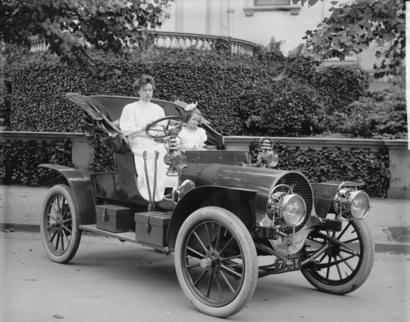
\includegraphics[width=\linewidth]{sample-franklin}
  \caption{1907 Franklin Model D roadster. Photograph by Harris \&
    Ewing, Inc. [Public domain], via Wikimedia
    Commons. (\url{https://goo.gl/VLCRBB}).}
  \Description{The 1907 Franklin Model D roadster.}
\end{figure}



\subsection{The ``Teaser Figure''}

A ``teaser figure'' is an image, or set of images in one figure, that
are placed after all author and affiliation information, and before
the body of the article, spanning the page. If you wish to have such a
figure in your article, place the command immediately before the
\verb|\maketitle| command:
\begin{verbatim}
  \begin{teaserfigure}
    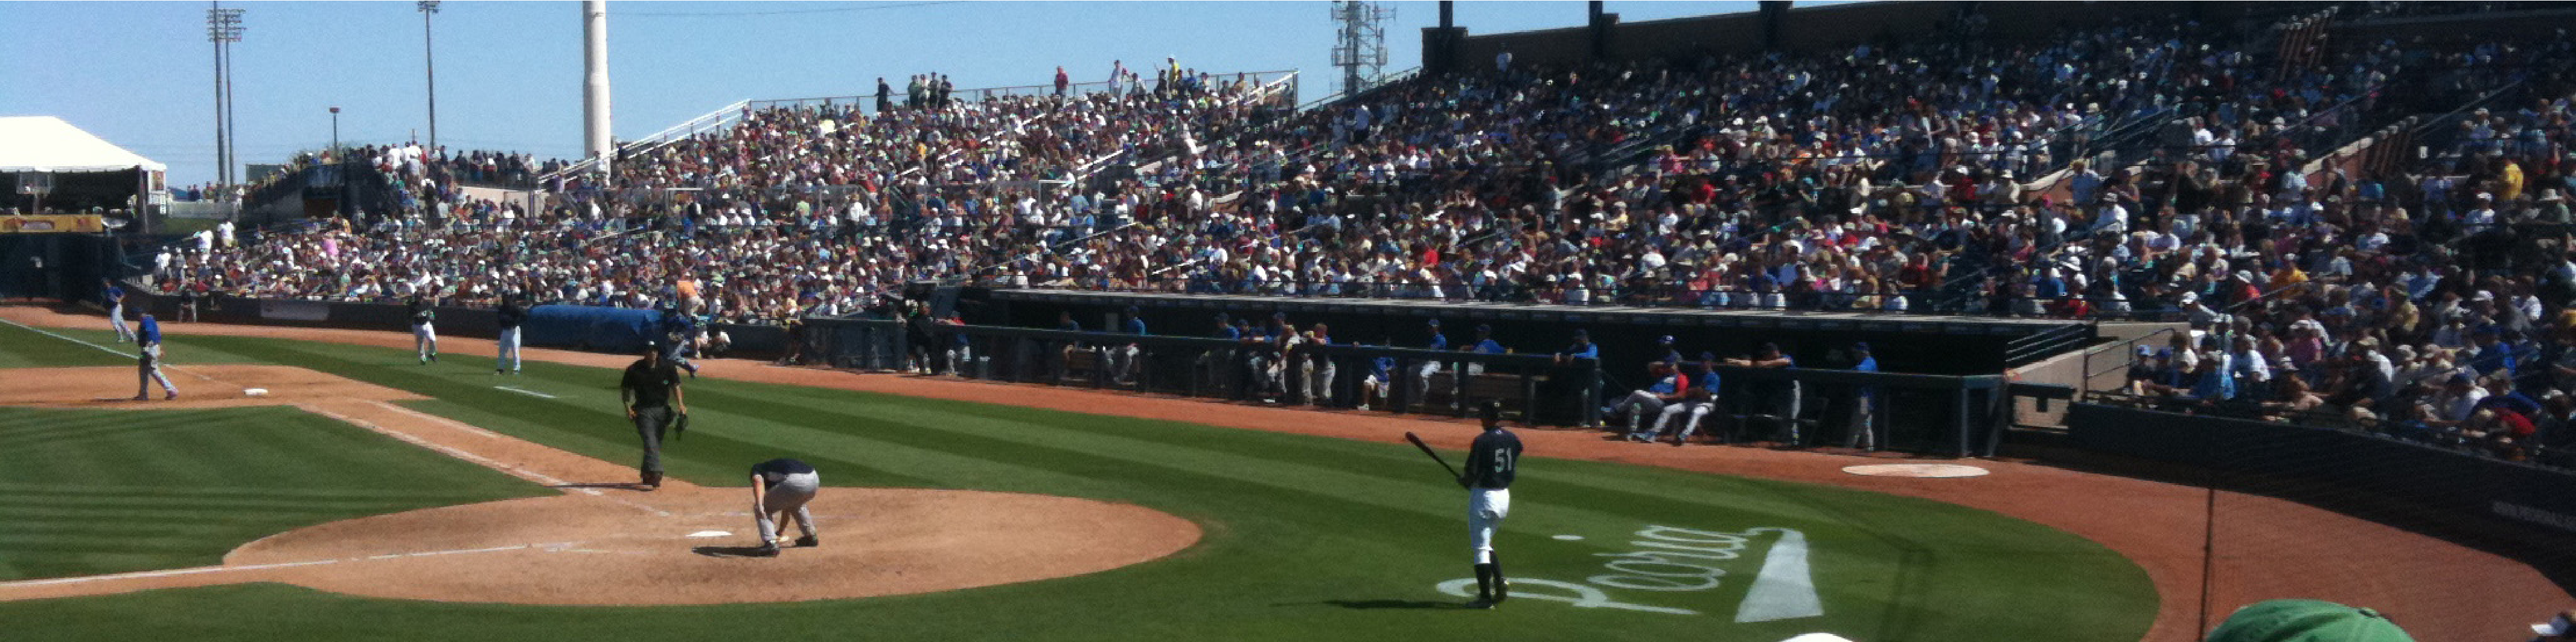
\includegraphics[width=\textwidth]{sampleteaser}
    \caption{figure caption}
    \Description{figure description}
  \end{teaserfigure}
\end{verbatim}

\section{Citations and Bibliographies}

The use of \BibTeX\ for the preparation and formatting of one's
references is strongly recommended. Authors' names should be complete
--- use full first names (``Donald E. Knuth'') not initials
(``D. E. Knuth'') --- and the salient identifying features of a
reference should be included: title, year, volume, number, pages,
article DOI, etc.

The bibliography is included in your source document with these two
commands, placed just before the \verb|\end{document}| command:
\begin{verbatim}
  \bibliographystyle{ACM-Reference-Format}
  \bibliography{bibfile}
\end{verbatim}
where ``\verb|bibfile|'' is the name, without the ``\verb|.bib|''
suffix, of the \BibTeX\ file.

Citations and references are numbered by default. A small number of
ACM publications have citations and references formatted in the
``author year'' style; for these exceptions, please include this
command in the {\bfseries preamble} (before
``\verb|\begin{document}|'') of your \LaTeX\ source:
\begin{verbatim}
  \citestyle{acmauthoryear}
\end{verbatim}

  Some examples.  A paginated journal article \cite{Abril07}, an
  enumerated journal article \cite{Cohen07}, a reference to an entire
  issue \cite{JCohen96}, a monograph (whole book) \cite{Kosiur01}, a
  monograph/whole book in a series (see 2a in spec. document)
  \cite{Harel79}, a divisible-book such as an anthology or compilation
  \cite{Editor00} followed by the same example, however we only output
  the series if the volume number is given \cite{Editor00a} (so
  Editor00a's series should NOT be present since it has no vol. no.),
  a chapter in a divisible book \cite{Spector90}, a chapter in a
  divisible book in a series \cite{Douglass98}, a multi-volume work as
  book \cite{Knuth97}, an article in a proceedings (of a conference,
  symposium, workshop for example) (paginated proceedings article)
  \cite{Andler79}, a proceedings article with all possible elements
  \cite{Smith10}, an example of an enumerated proceedings article
  \cite{VanGundy07}, an informally published work \cite{Harel78}, a
  doctoral dissertation \cite{Clarkson85}, a master's thesis:
  \cite{anisi03}, an online document / world wide web resource
  \cite{Thornburg01, Ablamowicz07, Poker06}, a video game (Case 1)
  \cite{Obama08} and (Case 2) \cite{Novak03} and \cite{Lee05} and
  (Case 3) a patent \cite{JoeScientist001}, work accepted for
  publication \cite{rous08}, 'YYYYb'-test for prolific author
  \cite{SaeediMEJ10} and \cite{SaeediJETC10}. Other cites might
  contain 'duplicate' DOI and URLs (some SIAM articles)
  \cite{Kirschmer:2010:AEI:1958016.1958018}. Boris / Barbara Beeton:
  multi-volume works as books \cite{MR781536} and \cite{MR781537}. A
  couple of citations with DOIs:
  \cite{2004:ITE:1009386.1010128,Kirschmer:2010:AEI:1958016.1958018}. Online
  citations: \cite{TUGInstmem, Thornburg01, CTANacmart}. Artifacts:
  \cite{R} and \cite{UMassCitations}.



This section has a special environment:
\begin{verbatim}
  \begin{acks}
  ...
  \end{acks}
\end{verbatim}
so that the information contained therein can be more easily collected
during the article metadata extraction phase, and to ensure
consistency in the spelling of the section heading.

Authors should not prepare this section as a numbered or unnumbered {\verb|\section|}; please use the ``{\verb|acks|}'' environment.

%%
%% The next two lines define the bibliography style to be used, and
%% the bibliography file.
\bibliographystyle{ACM-Reference-Format}
\bibliography{sample-base}

\end{document}
\endinput
%%
%% End of file `sample-authordraft.tex'.
